\chapter{Related Work}

\section{Code-Size Optimisations}

Although initially motivated by performance, many of the classical optimisations achieve better performance by reducing code size.
A small code, besides having fewer instructions to execute, can also have a positive impact on the cache utilisation.
Classical optimisations that are effective in reducing code size include the elimination of redundant, unreachable, and dead code, as well as certain kinds of strength reduction~\cite{cocke70,briggs97,debray00}.
In this section, we will describe some of these classical size-reducing optimisations.

\subsection{Unreachable-Code Elimination}

Some functions may contain code that is unreachable. A code is unreachable if there is no valid control-flow path from the function's entry point that leads to it. Since unreachable code is guaranteed to never be executed, compilers should remove it to avoid code bloat.

Often, unreachable code is uncovered by other optimizations. For example, after constant propagation, a conditional branch could have its condition evaluating to a constant, eliminating a path to one of its successor basic block. If no other path leads to that basic block, it becomes unreachable.

The algorithm to eliminate unreachable code works in a mark-sweep manner, performing two passes over the basic blocks of the CFG. The reachability analysis optimistically assumes that all basic blocks are dead until proven otherwise. First, it marks all blocks as unreachable. Next, starting from the entry point, it marks each block that it can reach as reachable. If all branches and jumps are unambiguous, then all unmarked blocks can be deleted. With ambiguous branches or jumps, the compiler must preserve any block that the branch or jump can reach. This analysis is simple and inexpensive.

\subsection{Dead-Code Elimination}



\section{Merging Identical Functions}

In this section, we will discuss existing optimisations for merging identical functions.
Figure~\ref{fig:example-identical} illustrates how identical functions can appear in real programs.
The first pair of functions, shown in Figure~\ref{fig:example-identical-1-sphinx3}, were extracted from the \texttt{482.sphinx3} benchmark.
The only difference between these two functions is in their parameter type.
However, all pointer types can be considered equivalent since they can be bitcasted in a losslessly way.
These functions are usually produced by copy-and-paste programming, where a given code pattern is copied and then repurposed~\cite{kim04,jablonski10,ahmed15}.
The second pair of functions, shown in Figure~\ref{fig:example-identical-2-gcc}, were extracted from the \texttt{403.gcc} benchmark and they are fully identical.
These functions are part of GCC's backend, where it is common to have code that is automatically generated from a machine description~\cite{muchnick98,kolek13,ghica15}.

\begin{figure}[h]
\centering
\begin{subfigure}{\textwidth}
\centering
\includegraphics[scale=0.9]{src/relatedwork/figs/example-identical-1-sphinx3}
\caption{Two semantically identical functions extracted from the \texttt{482.sphinx3} benchmark.}
\label{fig:example-identical-1-sphinx3}
\end{subfigure}
\begin{subfigure}{\textwidth}
\centering
\includegraphics[scale=0.9]{src/relatedwork/figs/example-identical-2-gcc}
\caption{Two semantically identical functions extracted from the \texttt{403.gcc} benchmark.}
\label{fig:example-identical-2-gcc}
\end{subfigure}
\caption{Example of identical functions.}
\label{fig:example-identical}
\end{figure}

\begin{figure}[h]
\centering
\includegraphics[scale=0.9]{src/relatedwork/figs/identical-example}
\caption{Two function extracted from the \texttt{447.dealII} benchmark that are not identical at the source level, but after applying template specialisation and optimisations they become identical at the IR level.}
\label{fig:identical-example}
\end{figure}

Note, however, that functions can be identical at the IR or machine level without necessarily being identical at the source level.
Figure~\ref{fig:identical-example} shows two real functions extract from the
447.dealII program in the SPEC CPU2006~\cite{spec} benchmark suite.
Although these two functions are not identical at the source level, they become
identical after a template specialisation and some optimisations are applied, in
particular, constant propagation, constant folding, and dead-code elimination. 
Specializing \verb|dim| to $1$ enables to completely remove the loop in the
function \verb|PolynomialSpace|.
Similarly, specializing \verb|dim| to $1$ results in only the first iteration
of the loop in the function \verb|TensorProductPolynomials| being executed.
The compiler is able to statically analyze and simplify the loops in both
functions, resulting in the identical functions shown at the bottom of
Figure~\ref{fig:identical-example}.

Identical code is particularly common in C++ programs
with heavy use of \textit{parametric polymorphism}, via template or \textit{auto} type deduction.



\subsection{Merging Identical Object Code During Link Time}

The simplest way of merging identical functions is by looking at their object code, during link time.
\textit{Identical code folding}~(ICF) is an optimisation that identifies and merges two or more read-only sections, typically functions, that have identical contents.
This optimisation is commonly found in major linkers, such as \textit{gold}~\cite{tallam10,kwan12}, LLVM's \textit{lld}, and the MSVC linker~\cite{msvc-icf}.

Before applying ICS, it is a common practice for linkers to place functions in separate sections~\cite{tallam10,kwan12}.
Therefore, merging identical functions can be generalised to the problem of merging identical sections.
In the simplest case, two functions or sections are identical if they have exactly the same binary representation.
In general, two sections are considered identical if they have the identical section flags, data, code, and relocations.
Two relocations are considered identical if they have the same relocation types, values, and if they point to the same or, recursively, identical sections.

% Most object file formats, such as the \textit{Executable and Linkable Format} (ELF)~\cite{tallam10,kwan12}, are structured as separate sections of content, each section containing a certain type of content.
% The main types are code segment, different types of data segment, and relocation information.
% Relocation information describes how to modify other sections, connecting symbolic references to their definition.
% In other words, it assigns actual addresses for position-dependent code and data.
% For example, when a program calls a function, the associated call instruction must transfer control to the proper destination address at execution.

Once a set of identical functions have been identified, merging them requires a simple operation.
Only one of the functions in the set is kept for the final binary and all the other copies are discarded.
Afterwards, every reference to the discarded functions must be redirected to the kept function.
%We then map the symbols corresponding to the duplicate functions to have the same value as the symbol of the kept function.

% This is a trivial operation and the main challenge lies on the search strategy. 

% Figure~\ref{fig:icf-example} shows an example, adapted from Tallam~\etal~\cite{tallam10},
% of how generic programming in C++ can lead to identical functions in the object file.
% The C++ code in in Figure~\ref{fig:icf-example-code} presents
% a simple \textit{template class} and its member function being
% instantiated multiple times with different pointer types.
% Figure~\ref{fig:icf-example-object} shows the object code 
% targeting the Intel x86 architecture.
% For each instantiation of \textit{Foo}, a replica of its member
% function \textit{getElement} is created.
% Because the size of the different pointer types is the same,
% all replicas of \textit{getElement} are identical
% in the object file, which can be easily confirmed by
% comparing their binary representation. as shown in
% Figure~\ref{fig:icf-example-object}.

% \begin{figure}[h]
% \begin{tabular}{cc}
% \begin{subfigure}{.5\textwidth}
% \includegraphics[scale=0.9]{src/relatedwork/figs/icf-example-1}
% \caption{A \textit{template class} with several instantiations.}
% \label{fig:icf-example-code}
% \end{subfigure} &
% \begin{subfigure}{.5\textwidth}
% \includegraphics[scale=0.9]{src/relatedwork/figs/icf-example-2}
% \caption{Disassembled object file.}
% \label{fig:icf-example-object}
% \end{subfigure}
% \end{tabular}
% \caption{Example showing how a member function of a \textit{template class}
%   can produce code replication susceptible to \textit{identical code folding}.
%   For each instantiation of \textit{Foo}, a replica of the function
%   \textit{getElement} is created for the template instance.
%   When instantiated with pointer types, the object code of these functions will be identical.}
% \label{fig:icf-example}
% \end{figure}

Since the equality relation has a cyclic definition, ICF is defined as a fixed-point computation, i.e., it is applied repeatedly until a convergence is obtained.
There are two approaches with distinct trade-offs:
$(i)$ The pessimistic approach starts with all sections marked as being different and then repeatedly compare them trying to prove their equality, grouping those found to be identical, including their relocations.
This approach is implemented in the widely used \textit{gold} linker.
$(ii)$ The optimistic approach starts with all functions marked as potentially identical and then repeatedly compare trying to disprove their equality, partitioning those found to be different.
This approach is implemented in LLVM's linker, \textit{lld}.


% \subsection{The Pessimistic Algorithm}

% The pessimistic algorithm is implemented in the \textit{gold} linker.
% It starts by marking all functions as different and repeatedly compute their checksum to identify and merge more identical functions.
% This has the advantage that the algorithm can stop at any iteration, before the actual convergence, and correctness will be guaranteed.
% By limiting the number of iterations, regardless of convergence, we are essentially limiting the compilation-time overhead, potentially missing some optimisation opportunities.

% We can start with marking all functions as different and repeatedly do
% the checksumming.  This has the advantage that we do not need to wait
% for convergence. We can stop at any point and correctness will be
% guaranteed although not all cases would have been found.  However, this
% has a problem that some cases can never be found even if it is run until
% convergence.  Here is an example with mutually recursive functions :

% int funcA (int a)            int funcB (int a)
% {                            {
%   if (a == 1)                  if (a == 1)
%     return 1;                    return 1;
%    return 1 + funcB(a - 1);     return 1 + funcA(a - 1);
% }                            }

% In this example funcA and funcB are identical and one of them could be
% folded into the other.  However, if we start with assuming that funcA
% and funcB are not identical, the algorithm, even after it is run to
% convergence, cannot detect that they are identical.


% \subsection{The Optimistic Algorithm}

% The optimistic algorithm is implemented in LLVM linker, lld.

% \begin{figure}[h]

% \begin{subfigure}{\textwidth}
% \centering
% \includegraphics[width=0.9\textwidth]{src/relatedwork/figs/icf-example-code}
% \caption{.}
% \label{fig:identical-example-code}
% \end{subfigure}

% \begin{subfigure}{\textwidth}
% \centering
% \includegraphics[width=0.9\textwidth]{src/relatedwork/figs/icf-example-diagram}
% \caption{.}
% \label{fig:identical-example-diagram}
% \end{subfigure}

% \caption{Example showing how a member function of a \textit{template class}
%   can produce code replication susceptible to \textit{identical code folding}.
%   For each instantiation of \textit{Foo}, a replica of the function
%   \textit{getElement} is created for the template instance.
%   When instantiated with pointer types, the object code of these functions will be identical.}
% \label{fig:icf-example}
% \end{figure}


\section{Identical Code Folding in Linkers}

Google developed an optimisation for the \textit{gold} linker that merges
identical functions on a bit-level~\cite{tallam10,kwan12}.
After placing each function in a separate ELF section, they identify function
sections that have their \textit{text} section bit-identical and also their
relocations point to sections that are identical. A simpler version of this
optimisation was also offered by the MSVC linker~\cite{msvc-icf};

\section{Identical Function Merging}

A similar optimisation for merging identical functions, but instead at the
intermediate representation (IR) level, is also offered by both GCC and
LLVM~\cite{llvm-fm,livska14}.
%The function merging optimisation currently offered by LLVM is only able to
%merge identical functions.
This optimisation is only flexible enough to accommodate simple type mismatches
provided they can be bitcasted in a losslessly way.
%Similarly to the technique proposed by Edler von Koch~et~al.~\cite{edler14},
%LLVM's optimisation also exploits structural similarity among functions.
%However, the current implementation does not allow instructions to differ in
%their opcodes or in the number and type of their input operands.
Although very restrictive, this optimisation guarantees that any pair of
mergeable functions will result in code size reduction with no performance
overhead.
%Its simplicity also benefits compilation time, as the actual merge operation
%is trivial.
Its simplicity also allows for an efficient exploration approach based on computing
a hash of the functions and then using a binary tree to identify equivalent
functions.

%%%%%%%%%%%%%%%%%%%%%%%%%%%%%%%%%%%%%%%%%%%%%%%%%%%%%%%%%%%%%%%%%%%%%%%%%%%%%%%%

%We define a congruent group as a set of functions that are candidates for
%function equality.
%To create congruent groups, we build a compound hash value for each previously
%parsed function.
%%%As an optimisation, a hash of the function structure is calculated first, and
%%%two functions are only compared if they have the same hash.

Since hashing is cheap to compute, it allows us to efficiently
%Hashing is used to
group possibly equivalent functions and filter out functions
that are guaranteed to be unique.
%This hash is cheap to compute,
This hash must have the property that if function $F = G$
according to the comparison function, then $hash(F) = hash(G)$.
Therefore, as an optimisation, two functions are only compared if they have the
same hash.
This consistency property is critical to ensuring all possible merging
opportunities are exploited.
Collisions in the hash affect the speed of the pass but not the correctness
or determinism of the resulting transformation.

A function hash is calculated by considering only the number of arguments and
whether a function is varargs, the order of basic blocks (given by the
successors of each basic block in depth first order), and the order of
opcodes of each instruction within each of these basic blocks. This mirrors
the strategy compare() uses to compare functions by walking the BBs in depth
first order and comparing each instruction in sequence. Because this hash
does not look at the operands, it is insensitive to things such as the
target of calls and the constants used in the function, which makes it useful
when possibly merging functions which are the same modulo constants and call
targets.

After that, the pass sorts each function to a congruent class according to
its hash value.
All functions in the module, ordered by hash. Functions with a unique
hash value are easily eliminated.
If the hash value matches the previous value or the next one, we must
consider merging it. Otherwise it is dropped and never considered again.

The functions that remain are inserted into a binary tree, where functions are
the node values themselves.
An order relation is defined over the set of functions.
We need total-ordering, so we need to maintain four properties on the functions set:
\begin{itemize}
\item $a <= a$ (reflexivity);
\item if $a <= b$ and $b <= a$ then $a = b$ (antisymmetry);
\item if $a <= b$ and $b <= c$ then $a <= c$ (transitivity);
\item for all $a$ and $b$, $a <= b$ or $b <= a$ (totality).
\end{itemize}
This total-ordering was made through special function comparison procedure that
returns:
\begin{itemize}
\item 0 when functions are semantically equal,
\item -1 when Left function is less than right function, and
\item 1 for opposite case.
\end{itemize}
This function comparison iterates through each instruction in each basic block.
The FunctionComparator compares two functions to determine whether or not
they will generate machine code with the same behaviour. DataLayout is
used if available. The comparator always fails conservatively (erring on the
side of claiming that two functions are different).


After the previous step is finished, all candidates in a group must be proved to
be really semantically equivalent.

First it Compares the signature and other general attributes of the two functions.
The functions must have identical signature, i.e., the same return type, the same
number of arguments, and the same list of argument types, preserving argument order.
Then they do a CFG-ordered walk since the actual ordering of the blocks in the
linked list is immaterial. This walk starts at the entry block for both
functions, then takes each block from each terminator in order. As an
artifact, this also means that unreachable blocks are ignored.
Finally, two blocks are equivalent if they have equivalent instructions in
exactly the same order.

Functions are kept on binary tree. For each new function F we perform
lookup in binary tree.

%Therefore, by construction, functions are hashed and grouped in O(n log n) time
%complexity.


If we encounter a pair of functions as a candidate for merge, we can create either
an alias or thunk (function wrapper). We prefer to do an alias, which is cheaper
and merging is applied according to following rules:
1. If the address of at least one function is not taken, alias can be used.
2. But if the function is part of COMDAT section that can be replaced, we
must use thunk.
3. If we create a thunk and none of functions is writeable, we can redirect calls
instead.




\section{Merging Beyond Identical Functions}

In the previous sections, we have seen compiler optimisations that merge identical functions.
However, nearly identical functions, with only minor differences, are also commonly found.
Figure~\ref{fig:example-similar} shows two examples of nearly identical functions found in real programs.
The highlighted differences prevent these functions from being merged by the identical function merging techniques.
%These functions are usually produced by copy-and-paste programming,
%where a given code pattern is copied and then repurposed~\cite{kim04,jablonski10,ahmed15}.
The first pair of functions, shown in Figure~\ref{fig:example-similar-1-hmmer}, illustrates code that is usually produced by copy-and-paste programming,
where a given code pattern is copied and then repurposed~\cite{kim04,jablonski10,ahmed15}.
The second pair of functions, shown in Figure~\ref{fig:example-similar-3-gcc}, are produced by generative programming~\cite{czarnecki99,draheim04}, where their code was
automatically generated using a description language~\cite{ghica15}.

\begin{figure}[h]
\centering
\begin{subfigure}{\textwidth}
\centering
\includegraphics[width=0.9\textwidth]{src/relatedwork/figs/example-similar-1-hmmer}
\caption{Two similar functions extracted from the \texttt{456.hmmer} benchmark.}
\label{fig:example-similar-1-hmmer}
\end{subfigure}
%\begin{subfigure}{\textwidth}
%\centering
%\includegraphics[width=0.9\textwidth]{src/relatedwork/figs/example-similar-2-gcc}
%\caption{Two similar functions extracted from the \texttt{403.gcc} benchmark.}
%\label{fig:example-similar-2-gcc}
%\end{subfigure}
\begin{subfigure}{\textwidth}
\centering
\includegraphics[width=0.9\textwidth]{src/relatedwork/figs/example-similar-3-gcc}
\caption{Two similar functions extracted from the \texttt{403.gcc} benchmark.}
\label{fig:example-similar-3-gcc}
\end{subfigure}
\caption{Example of }
\label{fig:example-similar}
\end{figure}

Von Edler~et~al.~\cite{edler14} have proposed a function-merging technique exploits structural similarity among functions.
Their optimization is able to merge similar functions that are not necessarily
identical.
Two functions are structurally similar if both their function types are equivalent
and their CFGs isomorphic.
Two function types are equivalent if they agree in the number, order, and types
of their parameters as well as
their return types, linkage type, and other compiler-specific properties.
In addition to the structural similarity of the functions, their technique also
requires that corresponding basic blocks have exactly the same number of instructions
and that corresponding instructions must have equivalent resulting types.
% but may differ in their opcodes or in the number and type of their input operands.
Mergeable functions are only allowed to differ in corresponding instructions,
where they can differ in their opcodes or in the number and type of their input operands.
%The only differences that are actually allowed is that
%corresponding instructions can 
%differ in their opcodes or in the number and type of their input operands.

%If two corresponding instructions have different opcodes, they split the basic
%block and insert a switch branch to select which instruction to execute
%depending on a function identifier.

Because the state-of-the-art is limited to functions with identical CFGs
and function types, once it merges a pair of functions, a third
\textit{similar} function cannot be merged into the resulting merged function
since they will differ in both CFGs and their lists of parameters.
Due to this limiting factor, the state-of-the-art has to first collect all
mergeable functions and merge them simultaneously.

The state-of-the-art algorithm iterates simultaneously over corresponding basic
blocks in the set functions being merged, as they have isomorphic CFGs.
For every basic block, if their corresponding instructions have different opcodes,
they split the basic block and insert a switch branch to select which instruction
to execute depending on a function identifier.
Because these instructions have equivalent resulting types, their results can be
merged using a phi-operator, which can then be used transparently as operands
by other instructions.

Although the state-of-the-art technique improves over LLVM's identical function merging, it is
still unnecessarily limited. In Section~\ref{sec:motivation}, we showed examples of very similar
real functions where the state-of-the-art fails to merge. Our approach addresses such limitations
improving on the state-of-the-art across the board.




\textbf{TODO: Comparison table: Identical vs VonKoch vs Ours}


\section{Code Factoring}

%Function merging and code factoring are different techniques for solving the
%same fundamental problem of duplicated code.
Code factoring refer to related techniques that address the same fundamental
problem of duplicated code in a different way.
%While the former works by merging similar functions, the latter works by
%factoring out duplicated code~\cite{loki04}.
%Instead of merging similar functions, code factoring works by factoring out
%duplicated code into separate functions~\cite{loki04}.
Code factoring can be applied at different levels of the program~\cite{loki04}.
Local factoring, also known as local code motion, moves identical instructions
from multiple basic blocks to either their common predecessor or successor,
whenever valid~\cite{knoop94,briggs94,loki04}.
Procedural abstraction %(or outlining)
finds identical code
that can be extracted into a separate function, replacing all replicated
occurrences with a function call~\cite{loki04,dreweke07}.

Procedural abstraction differs from function merging as it usually works on
single basic blocks or single-entry single-exit regions.
Moreover, it only works for identical segments of code, and every identical
segment of code is extracted into a separate new function.
Function merging, on the other hand, works on whole functions, which can be
identical or just partially similar, producing a single merged function.

However, all these techniques are orthogonal to the proposed optimization and
could complement each other at different stages of the compilation pipeline.




\section{Code Similarity}

Code similarity has also been used in other compiler optimizations or tools for
software development and maintenance.
In this section, we describe some of these applications.

Coutinho~et~al.~\cite{coutinho11} proposed an optimization that uses instruction
alignment to reduce divergent code for GPU.
They are able to fuse divergent branches that contain single basic blocks,
improving GPU utilization.
%reducing idle cores.

Similarly, analogous algorithms have also been suggested to identify the
differences between two programs, helping developers with source-code
management and maintenance~\cite{yang91,miller85}.
These techniques are applied in tools for source-code management, such as
the \textit{diff} command~\cite{miller85}.

Similar techniques have also been applied to code editors and IDEs~\cite{toomim04,sajnani16}.
For example,
SourcererCC~\cite{sajnani16} detects possible clones, at the source level, by
dividing the programs into a set of code blocks where each code block is itself
represented by a bag-of-tokens, i.e., a set of tokens and their frequencies.
Tokens are keywords, literals, and identifiers, but not operators.
Code blocks are considered clones if their degree of similarity is higher than
a given threshold.
In order to reduce the number of blocks compared, candidate blocks are filtered
based on a few of their tokens where at least one must match.

Our ranking mechanism uses an approach similar to SourcererCC, where we use
opcode frequencies and type frequencies to determine if two functions are
likely to have similar code.
However, we need a precise and effective analysis of code similarity when
performing the actual merge.
To this end, we use a sequence alignment technique.




